\chapter{Background}\label{chapter:background}

This chapter will give insights into the most important topics and technologies relevant to this thesis. At the beginning, the topic of software monoliths is briefly introduced. The following section is about the abstraction of \acp{API} focusing on \acp{BFF}. Afterwards, the micro-frontend architecture is described with its characteristics, advantages, and disadvantages. Then the section explains different integration strategies as well as communication patterns. The section also goes into the topic of Generic \acp{API} vs. Consumer Driven \acp{API}. Next, a brief overview of GraphQL's characteristics, advantages, and disadvantages is given. Then the section describes implementations of GraphQL specification in the form of Apollo Server and Apollo Client. Particular importance is attached to explaining how the Apollo Client's in-memory cache works. In the end, the chapter briefly describes how removing fields from a GraphQL query with a caching mechanism could work in theory.

\section{Software Monoliths}\label{section:background:software-monolith}

A monolithic architecture is characterized that there is only one single codebase. Many developers, regardless of which team, are working on the same application. This approach to development was the standard for a very long time and is well supported by various modern development tools. By just having one application, the developers have an overview of the entire application. This software development approach uses a single database with one schema. A prototypical architecture for a monolithic application is shown in Figure \ref{fig:background:monolith:monolith-sketch}.

\ifshowImages
\begin{figure}[H]
  \centering
  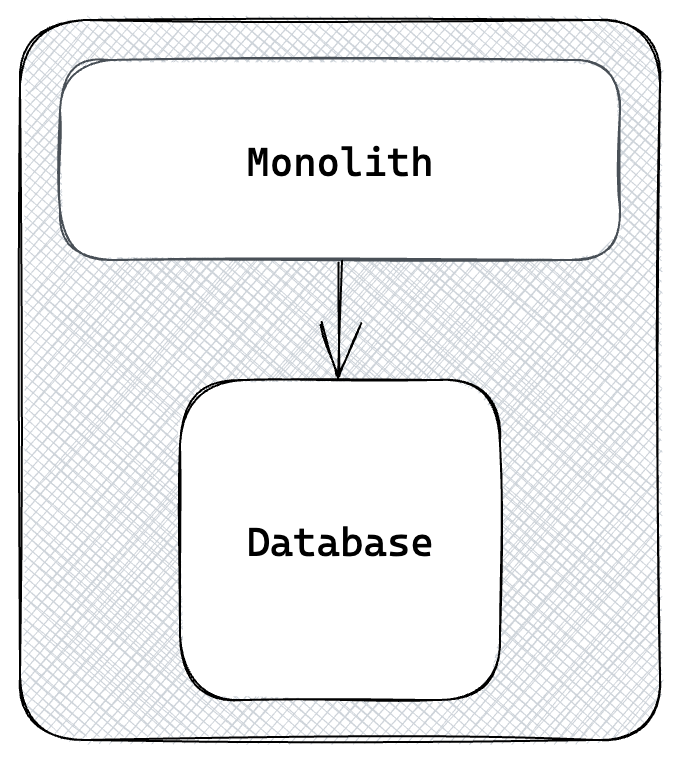
\includegraphics[width=0.3\linewidth]{images/background/monolith/monolith-sketch.png}
  \caption{The typical architecture of a software monolith. (Adapted from \cite[12]{book:2019:newman:background:monolith:monolith-to-microservices})}\label{fig:background:monolith:monolith-sketch}
\end{figure}
\fi

\bigskip

\noindent With a monolith, applying drastic changes to the complete codebase is easier. Modern \acp{IDE} support refactoring properties, for example, over the complete project. Therefore it is relatively easy to apply changes to every layer of the application, even the database schema. All project parts can be tested directly by running the application and the related database. Moreover, the complete application can be built and deployed in one step. Furthermore, it is easy to scale, as multiple instances can be run behind a load balancer. \cite[4]{book:2018:richardson:background:bff:microservices-patterns}

\bigskip

\noindent If a monolith starts to grow in size, it is essential to have a good software architecture. The code should be put in modules that follow the rules of high cohesion and low coupling of source code. The modularization splits the code into multiple chunks, which are easier to understand, but the application is still just a single process. Modules can be developed separately, but the application has to be deployed as one unit. This approach requires the coordination of various development teams. \cite[12-13]{book:2018:richardson:background:bff:microservices-patterns} \cite[12-13]{book:2019:newman:background:monolith:monolith-to-microservices} An example of such architecture is shown in the Figure \ref{fig:background:monolith:module-monolith-sketch}.

\ifshowImages
\begin{figure}[H]
    \centering
    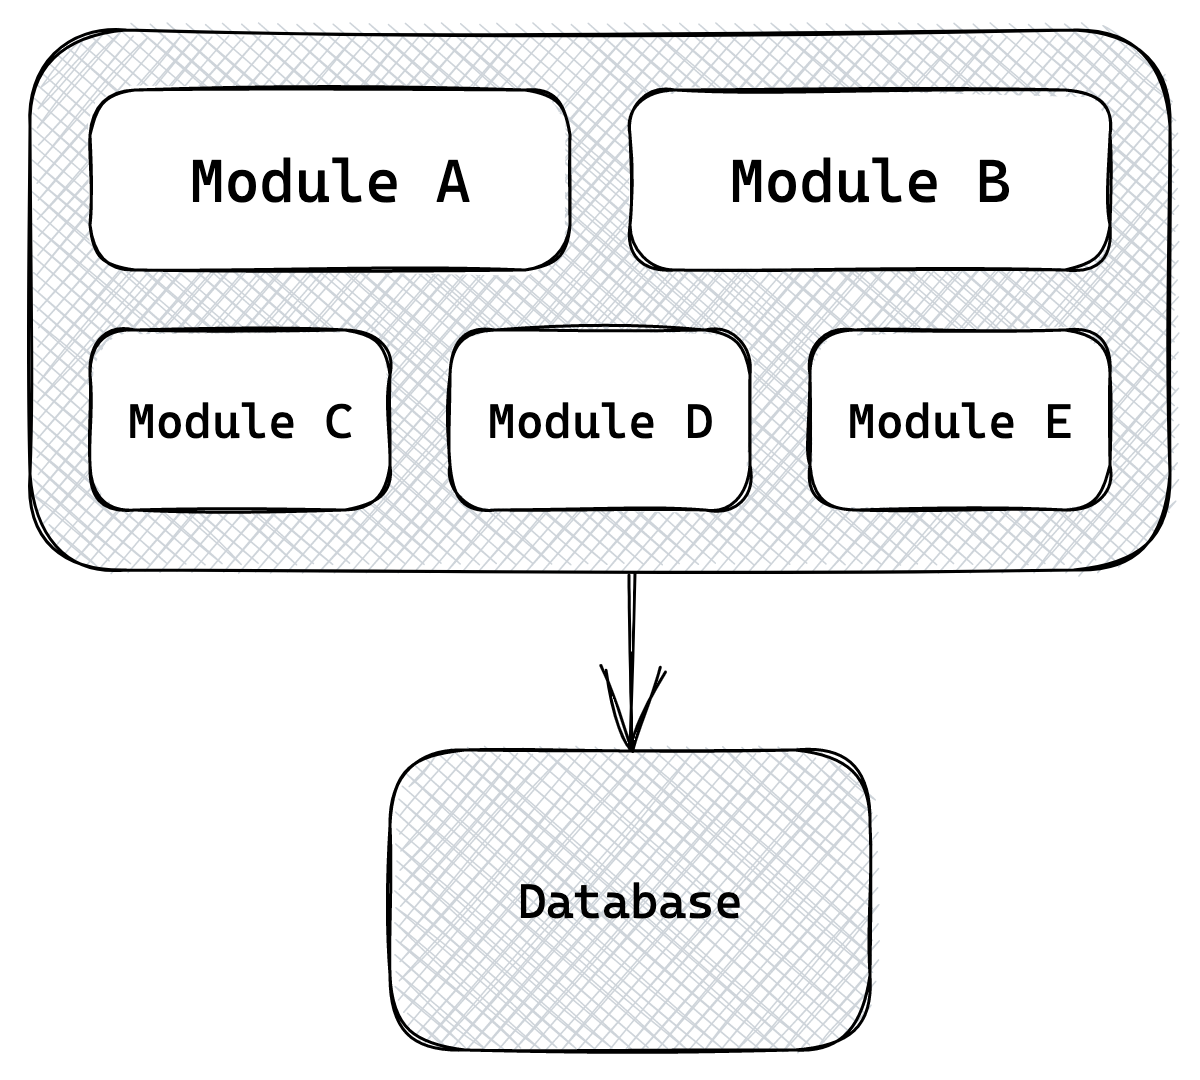
\includegraphics[width=0.4\linewidth]{images/background/monolith/modular-monolith-sketch.png}
    \caption{Structure of a modular monolith. (Adapted from \cite[13]{book:2019:newman:background:monolith:monolith-to-microservices})}\label{fig:background:monolith:module-monolith-sketch}
\end{figure}
\fi

\noindent Modular monoliths provide an excellent choice for many organizations. If there are well-defined module boundaries, parallel working is possible quite easily. However, a database cannot decompose the program logic into low-coupled modules like on the code level. \cite[12-13]{book:2019:newman:background:monolith:monolith-to-microservices}

\subsection{Disadvantages}\label{subsection:background:software-monolith:disadvantages}

With a growing code base, monolithic architectures come with increased complexity. Each new feature adds another complexity level, leading to reduced developer performance. Due to the existing entry hurdle, developing a new feature might be a very long process. The sheer size of the source code base makes it difficult to comprehend because program comprehension is an essential factor in software maintenance. \cite{article:1995:mayrhauser:background:monoliths:program-comprehension-during-software-maintenance-and-evolution} Therefore, developers might create side effects when fixing a bug. The time for developing a new feature increases drastically, and the internal architecture can also become challenging to understand and maintain. \cite[4-6]{book:2018:richardson:background:bff:microservices-patterns}

\bigskip

\noindent Another problem is that multiple teams might work on the same chunks of code. Two different developers might need to make a change to code in a shared library. A developer could change code inside a module, which he needs more information about. The change might also not be coordinated with other software engineers, which might lead to unexpected behavior in the other developer's code. The circumstance is also known as \textit{confused lines of ownership}, which are frequent sources of errors in a software system. \cite[15]{book:2019:newman:background:monolith:monolith-to-microservices} \cite[7]{inproceedings:2011:bird:background:monoliths:dont-touch-my-code}

\bigskip

\noindent With a monolithic approach, using different technologies is no longer possible, and the technology stack is restricted for the entire lifespan of the monolith. Introducing a different programming language or a different framework is impossible and often leads to a complete rewrite of an application. \cite[6-7]{book:2018:richardson:background:bff:microservices-patterns} The problem with technology is that it always becomes deprecated and obsolete at one point. Applications based on such deprecated technology must be reimplemented with a different programming language or framework. Simply rewriting the application in another framework is not straightforward because the application's functionality must be understood.

\subsubsection{Monolithic Systems are not Legacy Systems}\label{subsection:background:software-monolith:not-legacy-systems}

Developing a monolithic application should not be synonymous with writing a legacy application, and the term legacy application should not be used for monolithic systems. \cite[15]{book:2019:newman:background:monolith:monolith-to-microservices} The monolithic architecture is a good starting point for new applications. If some domains of the applications need to be better understood and when drastic changes can happen to already implemented features. It is easier to understand the complete application and make code changes. \cite[43]{book:2019:newman:background:monolith:monolith-to-microservices}


\section{API Abstraction Layer}

Every microservice provides its functionality to consumers with APIs. But it is not advisable that clients directly communicate with microservice APIs. Microservice offer fine-grained interfaces which were made especially for the communication between microservices. Therefore, the client usually has to make multiple requests to fetch the data and aggregate them to display a view inside the application. \cite{book:2021:newman:background:bff:micro-services} This leads to many requests, which is also known as over-requesting, which has a negative impact on the user experience. \cite{book:2018:richardson:background:bff:microservices-patterns}

% TODO: Progressive enhancement missing

Another problem could be that a cluster of microservices uses another form of communication. For example an asynchronous message-bus or another protocol like GRPC. Clients usually communicate using synchronous communication, where microservices might use asynchronous communication. Without an adapter in between, the communication will not work properly. Even if the communication is possible, the client needs to know many internal details about the cluster of microservices like the IP-address. It is not clear, which microservice offers the data that is needed for the client. Changing the API of a microservice would have a ripple effect on the requests on the frontends, because they would have to be changed in many places. \cite{book:2018:richardson:background:bff:microservices-patterns}

To solve this problem the clients communicate with an API gateway or a more client centric backend-for-frontend service. API gateways present an abstraction of a microservice APIs. It is the entry point to the system that is composed of multiple microservices. \cite{book:2020:siriwardena:background:bff:microservice-security-in-action}

The main task of a gateway is to forward tasks to the correct microservice and compose API for loading the needed data in one request. The even might implement functionalities like authorization and authentication or transform the protocol. Like transforming HTTP to GRPC. With API gateways it is also easier to split a microservice into two service, without a ripple effect to change all clients that consume that microservice as well. \cite{book:2018:richardson:background:bff:microservices-patterns}

But the problem with API gateways is the ownership. Multiple teams will add their functionality to the gateway and might come into conflict. The APIs are often not suited for the needs of clients and it has to be avoided that client logic is developed into the API gateway. Another pattern to bypass the problems with API gateways is the backend-for-frontend pattern. \cite{book:2018:richardson:background:bff:microservices-patterns}

With this approach each client application has its own API gateway, which is called backend-for-frontend service. This service is specially adapted for the needs of the client. \cite{book:2018:richardson:background:bff:microservices-patterns} \cite{book:2021:newman:background:bff:micro-services} This allows every team to develop their backend-for-frontend isolated and autonomous. Therefore a team can develop a complete vertical product starting from the microservice to the backend-for-frontend and finally the micro-frontend. \cite{book:2020:geers:background:micro-frontends:micro-frontends-in-action}

\subsection{Backend-for-frontend}


\section{Micro-Frontend Architecture}

Micro-frontends should bring the same advantages of microservices from the backend to the frontend. Instead of creating a large frontend monolith, a micro-frontend architecture contains many small applications. The advantage is that every micro-frontend can be developed and deployed by a separate team. \cite{book:2020:geers:background:micro-frontends:micro-frontends-in-action} The difference between frontend-monoliths and micro-frontends can be seen in figure \ref{figure:state-of-the-art:ui-monolith-micro-frontend}.

\ifshowImages
\begin{figure}[H]
\centering
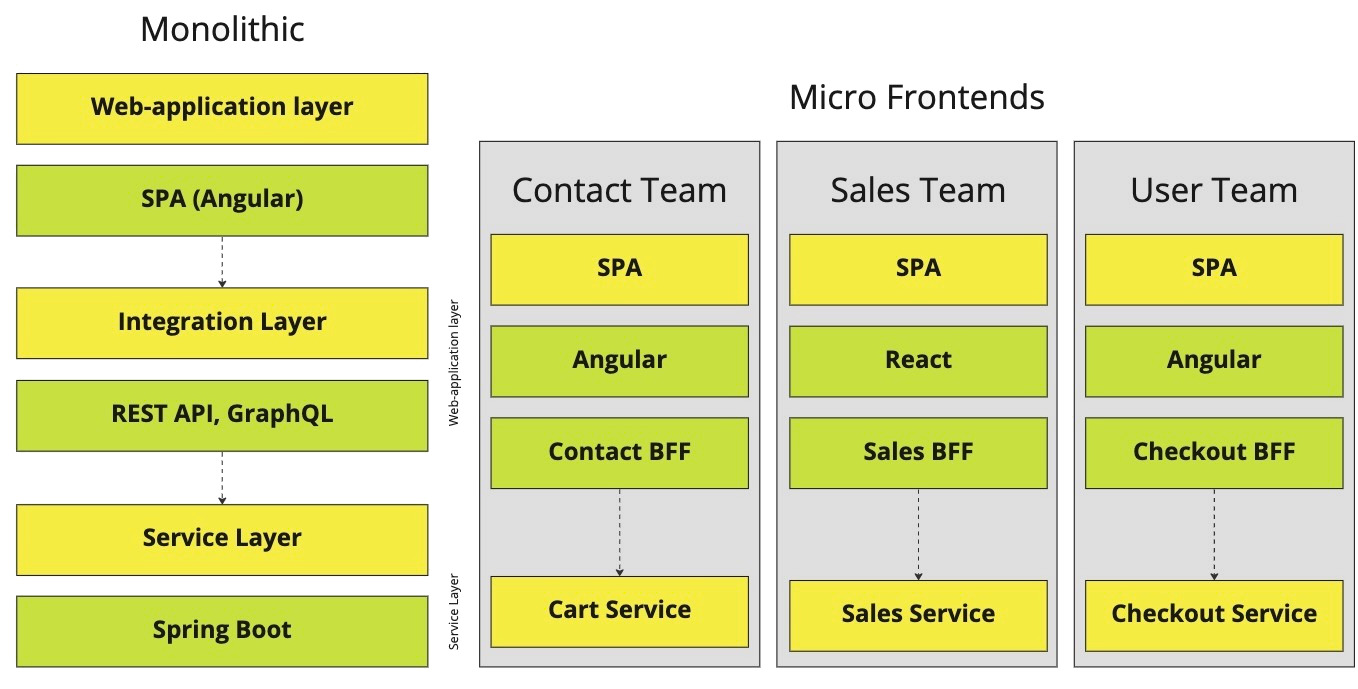
\includegraphics[width=0.8\linewidth]{images/ui-monolith-micro-frontends.jpeg}
\caption{A comparison between frontend-monoliths and micro-frontends.}\label{figure:state-of-the-art:ui-monolith-micro-frontend}
\end{figure}
\fi

Benefits gained from working with microservices on the backend are lost, when working with a monolithical frontend. With a monolithic frontend, the ability to deploy independently is lost. The entire frontend has to be deployed at once. Another problem is, that distinct operations are not really possible. If one part of the frontend is broken, there is a good chance that the entire frontend is broken. Another problem is the parallel development. The speed of development cannot be increased because it is very difficult to have multiple teams working on one frontend application. \cite{misc:2019:leitner:micro-frontends}

The term micro-frontend can be misleading, as can the term microservice. It has no meaning in terms of the size of the application. It can be a simple widget that only displays data, or a full-blown one-page application. Ideally, a micro frontend covers an area of the entire frontend application.


Micro-frontends try to apply the same principles from the microservice architecture to frontend development. Often times a microservice architecture with is developed by several teams has only one frontend application. Therefore, when adding new features a single team can be overwhelmed. Like a microservice architecture, a micro-frontend architecture focuses on developing many small frontend-applications, instead of developing a large software monolith. Each micro-frontend can be developed independently by another team. But a challenge is that the micro-frontend should appear as a single application to the user. Therefore, the different applications have to be integrated, which can be a challenge.

The term micro-frontend should not lead to false conclusions about the size of an application. The size of micro-frontends can vary. It can range from a simple login to a complex single-page application.

Building micro-frontends with the web allows different strategies of integrating the applications. Three different strategies exist to combine multiple micro-frontends into an app-shell. The client-side integration, the server-side integration and the combination of these two strategies and the combination of both strategies.

\subsection{Characteristics}

Micro-frontends tend to follow the same characteristics as microservices.

\subsubsection{Autonomous}

Technically a micro-frontend is a completely independent and runnable application. The integration of the micro-frontends happens only through the frontend. The different micro-frontends are composed withing an app-shell. The application shell is a separate application that is usually the entry-point for the user to interact with all micro-frontends. The app-shell also provides the layout of the page and defines where the micro-frontends are placed. The autonomy should not go in the direction of complete isolation. But no dependencies should emerge, which could the autonomy. \cite{book:2020:geers:background:micro-frontends:micro-frontends-in-action}

\subsubsection{Technology Agnostic}

Just as microservices architectures, micro-frontend architectures can be technology agnostic. The current frontend development landscape offers a lot of JavaScript frameworks to choose from. The advantage of an application that consists of small independent building blocks is that parts can be rewritten with another technology more easily. \cite{book:2020:geers:background:micro-frontends:micro-frontends-in-action} But using different technologies for different micro-frontends can lead to problems with the chosen form of integration and communication. The communication should be technology agnostic as well and should use browser native tools like Broadcast API.

Another problem that could arise is the bundle size of modern JavaScript frameworks. If two frameworks like React and Angular are fetched, the total bundle size can be very large and a strain for network connections. Loading an running multiple micro-frontends is also resource intensive. Due bypass this problem and offer a standardized API, micro-frontends can be developed with the help of Web Components. With this approach, no specific framework is needed to the application. \cite{book:2020:geers:background:micro-frontends:micro-frontends-in-action} 

\subsubsection{Independently Depoyable}

The autonomy of micro-frontends offer the possibility for independent deployments. A large monolithical frontend application is more complex to deploy. There is no need to have communication and coordination over multiple teams to deploy the application. Organizational dependencies have a negative impact on the time-to-market, because development teams would have to wait for the release of another team. \cite{book:2020:geers:background:micro-frontends:micro-frontends-in-action} 

\subsubsection{Small and Easy to Maintain}

Because micro-frontends only cover a small domain of an application, the source code is smaller and easier to understand. A smaller codebase is especially helpful for understanding the inner workings of software. 
Due to the easier understanding of the domain, the application can be easier rewritten with a state of the art technology, if the old one becomes deprecated. \cite{book:2020:geers:background:micro-frontends:micro-frontends-in-action}

\subsubsection{Resilience}

Micro-frontends offer the possibility to build an application by composing multiple independent applications into a fully fledged application. Depending on the integration strategy micro-frontends are usually combined at runtime. But the network, especially for mobile devices is not always without failures. A micro-frontend architecture provide better failure isolation. One micro-frontend crashing does not have an effect on the other micro-frontends inside the application. Some parts of the application might not work, but other parts of the application are still useable. The app-shell can react to a failure and tell users that the application is not working as expected and will be available back soon. \cite{article:2021:perltonen:background:micro-frontends:motivations-benefits-and-issues}

\subsection{Downsides of Micro-frontend architecture}

Due to the many advantages of micro-frontends there are also a downsides using this architectural approach. The independent development comes with the disadvantage of having redundancies. Each micro-frontend needs a separate build-process and also a continuous integration pipeline. And if the backend-for-frontend approach is, every micro-frontend needs it own backend-for-frontend service. It might happen that a lot of code is duplicated. when implementing this pattern. If multiple teams use the same code and a bug is found, the wrong behavior can't be fixed in a central place. Therefore, it is important to share knowledge between the teams to avoid running in the same bad situations over and over again. But this should not lead to inter-team dependencies between the different teams.
\cite{book:2020:geers:background:micro-frontends:micro-frontends-in-action} 


\subsection{Integration strategies}\label{subsection:background:micro-frontend-architecture:integration-strategies}

Micro-frontends can be integrated with different strategies. The integration strategy depends on the requirements of the system. They can be composed using a client-side integration strategy, a server-side strategy, or a combination of both.

\subsubsection{Server-Side Integration}\label{subsubsection:background:micro-frontend-architecture:integration-strategies:server-side-integration}

A Service between the client and the backend usually does server-side composition. \cite[60]{book:2020:geers:background:micro-frontends:micro-frontends-in-action} The server responds with references to micro-frontends that should be included and their required assets. The service in the middle intercepts that response and replaces the references to the micro-frontends with the actual content before the response is sent to the browser. The micro-frontends are included in their position and later appear in the HTML. An example of a server-side include can be seen in listing \ref{code:background:micro-frontends:server-side-include}. The other micro-frontends are referenced with URLs. \cite[61-63]{book:2020:geers:background:micro-frontends:micro-frontends-in-action}

\ifshowListings
\begin{listing}[H]
    \begin{minted}{html}
<html>
  <body>
    <!--#include virtual="/erp/dashboard" -->
  </body>
</html>
    \end{minted}
    \caption{An example server-side include.}\label{code:background:micro-frontends:server-side-include}
\end{listing}
\fi

\bigskip

\noindent One advantage of server-side integration is the fast first-load performance, which is the principle of progressive enhancement. \cite{book:2010:parker:background:micro-frontends:designing-with-progressive-enhancement} The browser fetches the HTML and renders it. It does not have to assemble parts of a page, like with client-side integration. The computation is only done on the server, which reduces the strain on the user's device. \cite{book:2020:geers:background:micro-frontends:micro-frontends-in-action} However, assets like stylesheets and images must still be fetched from the server. Server Side Integration is helpful if the application's primary concern is presenting static content to the end user and instant reaction to the users' inputs is unnecessary.  \cite[83]{book:2020:geers:background:micro-frontends:micro-frontends-in-action}

\subsubsection{Client-Side Integration}\label{subsubsection:background:micro-frontend-architecture:integration-strategies:client-side-integration}

When the application should react promptly to user input, a client-side integration strategy is preferred. For example, when developing an online marketplace, the user should be able to add items to the cart without making a complete roundtrip to the server to see the updated value. The application should provide a seamless user experience, as the end user just uses one application. Modern Frameworks like Angular and React offer the development of Single Page Applications, which provide reactive, client-side rendered applications. The HTML Markup is produced on the client instead of the server. \cite{book:2020:geers:background:micro-frontends:micro-frontends-in-action}

\bigskip

\noindent Client-side integration can be achieved through different approaches. The most straightforward approach combines the micro-frontends by linking the different applications with Hyperlinks. Each micro-frontend is deployed and accessible via a different URL, and the different micro-frontend applications are then linked with Hyperlinks. As the approach implies, switching to another micro-frontend requires a complete page reload and a roundtrip to the server. However, the integration with Hyperlinks breaks the SPA approach. This strategy makes it necessary that every micro-frontend is accessible via its URL and that it can be served as a standalone application.

\bigskip

\noindent Another client-side approach is to combine micro-frontend with iFrames or Web-Components. Integrating micro-frontends with this approach enables the page to be a SPA still. The client can navigate multiple micro-frontends without noticing, and no page reloads are needed. An iFrame is an isolated area with its own browser context \cite[35]{book:2020:geers:background:micro-frontends:micro-frontends-in-action}, Web Components are self-created HTML elements that are embedded into the DOM of the browser \cite[103]{book:2019:farrell:background:micro-frontends:web-components-in-action}. Integrating applications with the client-side strategy using Module Federation is explained in more detail in section \ref{subsubsection:background:micro-frontend:module-federation:101}.


\subsection{Communication between Micro frontends}

Micro-frontends should not depend on each other. But sometimes it is necessary have communication. For example if a user adds an item to the shopping-cart. The product micro-frontend has to inform the shopping-cart micro-frontend with the item that was added. The reduce the coupling between applications and development teams it is recommended to keep the communication at a minimum.

\subsection{Generic APIs vs Consumer Driven APIs}\label{subsection:background:micro-frontend:generic-vs-consumer-driven-apis}

The big decision in micro-frontend \ac{API} development is to use either generic or consumer-oriented \acp{API}. The difference is that generic \acp{API} emphasize reusability, while consumer-oriented \acp{API} tailor the \acp{API} to the customer.

\subsubsection{Generic \acp{API}}\label{subsubsection:background:micro-frontend:generic-vs-consumer-driven-apis:generic-apis}

Generic \acp{API} refer to \acp{API} that are very general and can be used by different clients. However, this type of \ac{API} has two significant drawbacks. Over-fetching describes the problem of getting more data than is needed, and Over-requesting describes the problem of needing multiple requests to get the data for a use case. Both problems are discussed in more detail in the following paragraphs. \cite{misc:2019:leitner:background:micro-frontends:backend-for-frontends}

\paragraph{Over-Fetching}\label{paragraph:background:micro-frontend:generic-vs-consumer-driven-apis:generic-apis:over-fetching}


For example, a contact service provides a contact model that includes \texttt{customerNumber}, \texttt{firstName}, \texttt{secondName}, \texttt{uidNumber}, and the user's address, as seen in the listing \ref{code:background:micro-frontends:over-fetching}. However, one application requirement is to display only a contact's first and last name inside the header. Only two fields of the model are used, and the rest are unnecessarily queried. \cite{misc:2019:leitner:background:micro-frontends:backend-for-frontends}

\ifshowListings
\begin{listing}[H]
    \begin{minted}{typescript}
interface ContactModel {
  id: string;
  customerNumber: string;
  firstName: string;
  secondName: string;
  uidNumber: string;

  Address: {
    id: string;
    postalCode: string;
    location: string;
    Country: string;
  }
}
    \end{minted}
    \caption{Contact-Model that contains too many fields for the requirement.}\label{code:background:micro-frontends:over-fetching}
\end{listing}
\fi

\paragraph{Over-Requesting}\label{paragraph:background:micro-frontend:generic-vs-consumer-driven-apis:generic-apis:over-requesting}

Attempting to solve the problem of over-fetching by reducing the amount of data set that is returned leads directly to this problem. Listing \ref{code:background:micro-frontends:over-requesting} shows the problem of over-requesting. If another requirement inside the application should display the address alongside the contact, two requests have to be performed every time. Afterwards, the two data sets have to be merged, leading to high client complexity. \cite{misc:2019:leitner:background:micro-frontends:backend-for-frontends}

\ifshowListings
\begin{listing}[H]
    \begin{minted}{typescript}
interface ContactModel {
  id: string;
  customerNumber: string;
  firstName: string;
  secondName: string;
  uidNumber: string;

  address_id: string;
}
    \end{minted}
    \caption{Contact-Model model that links the address-model with an id.}\label{code:background:micro-frontends:over-requesting}
\end{listing}
\fi

\subsubsection{Consumer Driven \acp{API}}\label{subsubection:background:micro-frontend:generic-vs-consumer-driven-apis:consumer-driven-apis}

Consumer-driven \acp{API} are the opposite of generic \acp{API}. They follow the idea of providing the client with exactly the data it needs. Following the example above, the contact service would have an endpoint that returns only the first and last name as required for the request. These endpoints make communication with a client straightforward, and there is no problem of over-fetching and over-requesting. However, creating an endpoint for each request creates an unmanageable set of endpoints.  \cite{misc:2019:leitner:background:micro-frontends:backend-for-frontends} To solve the problems of Over-fetching and Over-requesting, the \ac{BFF} pattern is often used. This pattern provides each client with their own \ac{API}, which is adapted to their needs. \cite{book:2018:richardson:background:bff:microservices-patterns}

\ifshowImages
\begin{figure}[H]
    \centering
    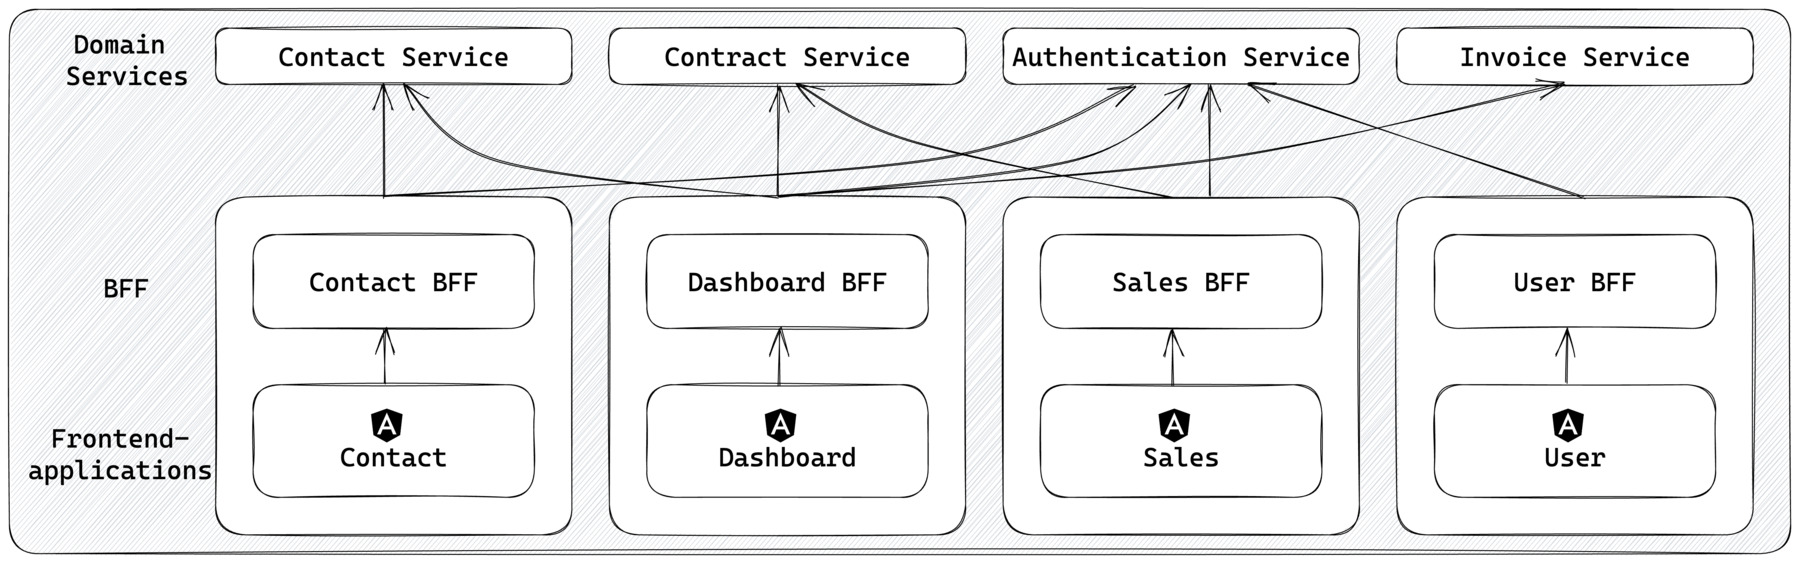
\includegraphics[width=1\linewidth]{images/background/micro-frontends/bff-architecture.jpg}
    \caption{Frontend architecture with the \ac{BFF} pattern.}\label{fig:background:micro-frontend:bff-architecture}
\end{figure}
\fi

\noindent Figure \ref{fig:background:micro-frontend:bff-architecture} shows an exemplary micro-frontend architecture using the \ac{BFF} pattern. Each frontend has a service that retrieves data only for that specific client. Because the \acp{BFF} function as a gateway to the domain services, the domain services can stay very generic and be reused by different clients. \acp{BFF} should implement only the presentation logic that puts the data into the form that the client needs, and it should avoid storing state. \cite{misc:2019:leitner:background:micro-frontends:backend-for-frontends}

\bigskip

\noindent With this architectural approach, the \ac{BFF} and the frontend form a single deployment unit. If one application changes, the other must adapt to the changes. GraphQL is a perfect technology for implementing a \ac{BFF} because it is specifically designed for implementing the presentation layer.


\section{GraphQL}\label{section:background:graphql}

GraphQL was initially developed by Facebook and refers to itself as the query language for \acp{API}. It allows the client to ask precisely for the data fields necessary. GraphQL offers the advantage that all requests can be fetched from only one endpoint. Data types provide an understandable implicit description of \ac{API} for consumers within the GraphQL schema. \cite{misc:-:background:graphql:graphql-org} The functionality of GraphQL can be compared to \ac{SQL} for databases. The client writes its queries with the desired fields from a query.

\bigskip

\noindent According to the official documentation, GraphQL is both a query language for \acp{API} and a runtime that executes those queries by using existing data. By providing a clear and comprehensive description of the data in the \ac{API}, GraphQL empowers clients to request only the data that they require, streamlining the data transfer process. This approach facilitates the evolution of \acp{API} over time and facilitates the development of powerful developer tools. The GraphQL specification is implemented in programming many languages and frameworks and has an extensive library and tool ecosystem.

\subsection{Origins and history}\label{subsection:background:graphql:origins-and-history}

GraphQL was initially developed in 2012. In 2015 the project was made open-source and available to the public. The reason behind the initial creation of GraphQL was the restricted flexibility of known \ac{API} technologies like \ac{REST}. Mobile devices needed only a subset of the fields that a \ac{REST} endpoint offered. Furthermore, the exact number of fields can change dynamically, based on the current state. The static background of \ac{REST} does not offer this behavior. Using \ac{REST}-based \acp{API} for clients that only need some fields would introduce the problem of over-fetching. Clients will be provided with information that exceeds their requirements. This approach leads to problems as mobile networks often have limited network traffic. Over-fetching puts additional strain on the user's data plan, as multiple requests have to be made. \cite{misc:2015:bryon:background:graphql:graphql-query-language}

\subsection{GraphQL Characteristics}\label{subsection:background:graphql:graphql-characteristics}

GraphQL has several design principles: \cite{misc:-:background:graphql:graphql-specification}

\begin{itemize}
  \item \textbf{Hierarchical}: Queries in GraphQL are structured hierarchically, allowing the clients to specify what data they need and in what format. This approach enables efficient data retrieval and reduces network overhead.

  \item \textbf{Product-centric}: GraphQL is designed to be product-centric rather than data-centric. That means that developers can create \acp{API} that match the needs of specific products or features rather than being constrained by the limitations of a pre-defined data schema.

  \item \textbf{Strong typing}: GraphQL is strongly-typed, meaning the data types are defined explicitly in the schema. The typing provides clarity and reduces ambiguity in the \ac{API} design while also enabling powerful tools for type checking and code generation.

  \item \textbf{Client-specified queries}: In GraphQL, the client specifies the structure of the query rather than the server. This approach allows clients to retrieve only the necessary data, reducing network overhead and enabling faster, more responsive applications.

  \item \textbf{Introspective}: GraphQL provides a built-in introspection system that enables clients to query the schema, allowing for powerful self-documentation and tooling capabilities.
\end{itemize}

\subsection{Advantages}\label{subsection:background:graphql:graphql-advantages}

GraphQL helps to reduce the network traffic between the clients and the service they query. Research indicates that the dynamic approach to fetching data can reduce the number of fields to be fetched and, therefore, the bytes sent back and forth to the GraphQL server. \cite{inprocessdings:2019:background:graphql:migration-to-graphql}

\bigskip

\noindent Because the client specifies the required fields that should be fetched, the complexity on the server can be reduced. The backend service does not need to implement many endpoints, that are only used by a small subset of clients. The \ac{API} can implement a single endpoint that all clients can query. \cite{book:2018:richardson:background:bff:microservices-patterns}

\bigskip

\noindent The characteristic that GraphQL can query its schema allows service discovery potential. Introspection allows GraphQL tools like GraphQL Voyager\footnote{\url{https://ivangoncharov.github.io/graphql-voyager/}} to visualize the schema in an \ac{UML} class diagram style. Other tools like GraphiQL\footnote{\url{https://github.com/graphql/graphiql}} can be used to analyze the schema and run queries. The functionality of such tools is explained in more detail in Section \ref{subsection:background:graphql:apollo-server-client}. \ac{REST} provides the same functionality to some degree, but additional tooling is needed because \ac{REST} cannot generate specification files.

\subsection{Disadvantages}\label{subsection:background:graphql:graphql-disadvantages}

\noindent The advantage that GraphQL reduces complexity on the server is a disadvantage for the client-side application. It leads to higher complexity when consuming GraphQL services compared to \ac{REST}. With \ac{REST}, only an endpoint has to be queried, whereas, with GraphQL, the requested data has to be specified at the field level. However, the introspection abilities of GraphQL allow consumers to understand better the query and data structure, which mitigates the disadvantage. A study \cite{inproceedings:2020:brito:background:graphql:rest-vs-graphql} showed that the study participants found it easier to consume a GraphQL Service than a \ac{REST} Service \cite{inproceedings:2017:de-pauda:background:graphql:handling-anti-patterns}. GraphQL shifts responsibilities from the server to the client, generally done with a gateway. \ac{API} composition can transfer the responsibility from the server to the client.

\bigskip

\noindent Allowing the client to specify the structure of a query might make the potential complexity of the query not transparent to the client. The approach makes it possibile that the client may specify a query which does not complete in a reasonable time or takes up a lot of resources. \cite{book:2018:richardson:background:bff:microservices-patterns}

\subsection{Apollo Server and Apollo Client}\label{subsection:background:graphql:apollo-server-client}

GraphQL has a specification and is a query language. Developing a GraphQL server and client is up to the application developer. Facebook has created its own GraphQL implementation of the specification in \ac{JS} with GraphQL.js for the backend and Relay for the frontend. Relay is a prominent example of a GraphQL client, but it is only available for Facebook's React framework. When evaluating different GraphQL clients, Apollo Client was chosen because it supports almost every possible programming language and framework.

\bigskip

\noindent Apollo Server is an open-source implementation of the GraphQL specification, and it offers any feature that the GraphQL specification states. Moreover, it supports Apollo Sandbox\footnote{\url{https://www.apollographql.com/docs/graphos/explorer/sandbox/}} out of the box. \cite{misc:-:background:graphql:apollo-server-introduction} Apollo Sandbox helps local development. Apollo Sandbox loads the GraphQL Schema from the server with the help of the Introspection Query. \cite{misc:-:background:graphql:apollo-sandbox} Such a development environment enables executing queries and mutations directly inside the browser.

\bigskip

\noindent Apollo Client is a community-driven project with npm packages for almost all frontend development environments like Angular, React, and Vue.js. The library fetches, caches, and manages the data of the application. The package for Angular is designed with Angular patterns in mind to integrate perfectly with the framework. Apollo Client offers the possibility to cache already made requests. \cite{misc:-:background:graphql:apollo-angular-client-overview} \cite{misc:-:background:graphql:apollo-client-overview} Caching is especially important as it can reduce the number of roundtrips to the server. The inner workings of the cache to prove or disprove the first hypothesis are explained in the following sections.

\subsubsection{How does the in-memory cache work?}\label{subsubsection:background:graphql:apollo-server-client:in-memory-cache-working}

This section describes how the caching mechanism of the Apollo Client works. The structure of the cache is a local, normalized, in-memory cache. All GraphQL requests made with Apollo Client are cached inside the browser's memory by default. The cache enables Apollo Client to respond almost immediately to queries for already-cached data without sending a network request. This mechanism is needed to reduce round-trips to the server in subsequent requests of the same query because the requested data can be served from the cache. \cite{misc:-:background:graphql:apollo-client-cache-overview} Caching mechanisms generally reduce the server's load but introduce issues with cache management.

\bigskip

\noindent \textbf{Apollo Client} includes a caching interface called \texttt{ApolloCache} and a proprietary implementation named \texttt{InMemoryCache}. Several Open-Source alternatives implement the \texttt{ApolloCache} interface, but Apollo's implementation is well-supported and receives regular updates.

\bigskip

\noindent Figure~\ref{fig:background:graphql:user-query-first-time} shows an exemplary query to fetch a user with its unique id. First, the Apollo Client checks whether the user with the given id is already stored inside the cache. If the query with that id has yet to be executed, a network query to fetch the user must be made. The result from the GraphQL Server is stored inside the cache and returned to the application. Four steps must be made to render data on the screen. \cite{misc:-:background:graphql:apollo-client-cache-overview}

\ifshowImages
\begin{figure}[H]
  \centering
  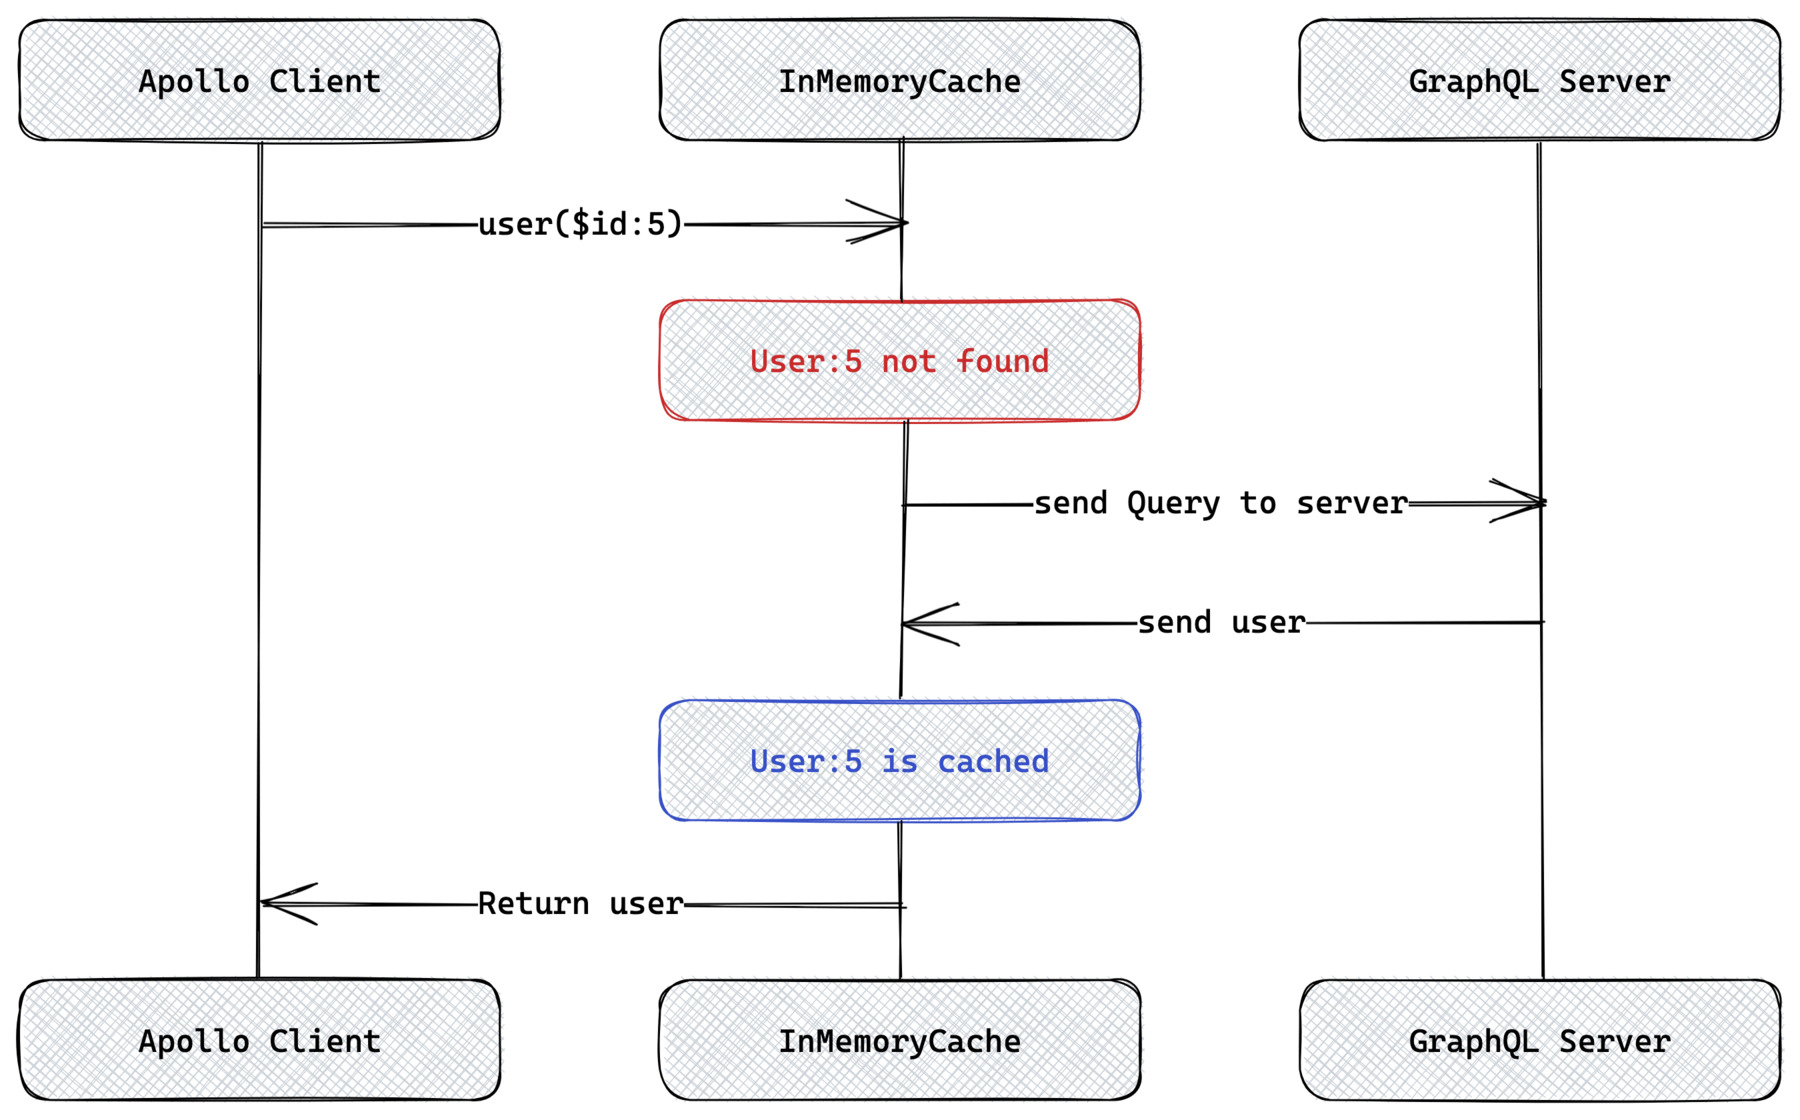
\includegraphics[width=0.6\linewidth]{images/background/graphql/apollo/apollo-client-basic-cache.jpg}
  \caption{The execution of a GraphQL query that is not stored in the cache. (Adapted from \cite{misc:-:background:graphql:apollo-client-cache-overview})}\label{fig:background:graphql:user-query-first-time}
\end{figure}
\fi

\noindent If a request with the same user id is made again, the flow of execution looks like in Figure \ref{fig:background:graphql:user-query-second-time}. As seen in the figure, no network request has to be made to the GraphQL \ac{API}, because everything is served from the Apollo Cache alone. Compared to the four steps in Figure \ref{fig:background:graphql:user-query-first-time}, only two steps need to be done here. \cite{misc:-:background:graphql:apollo-client-cache-overview}

\ifshowImages
\begin{figure}[H]
  \centering
  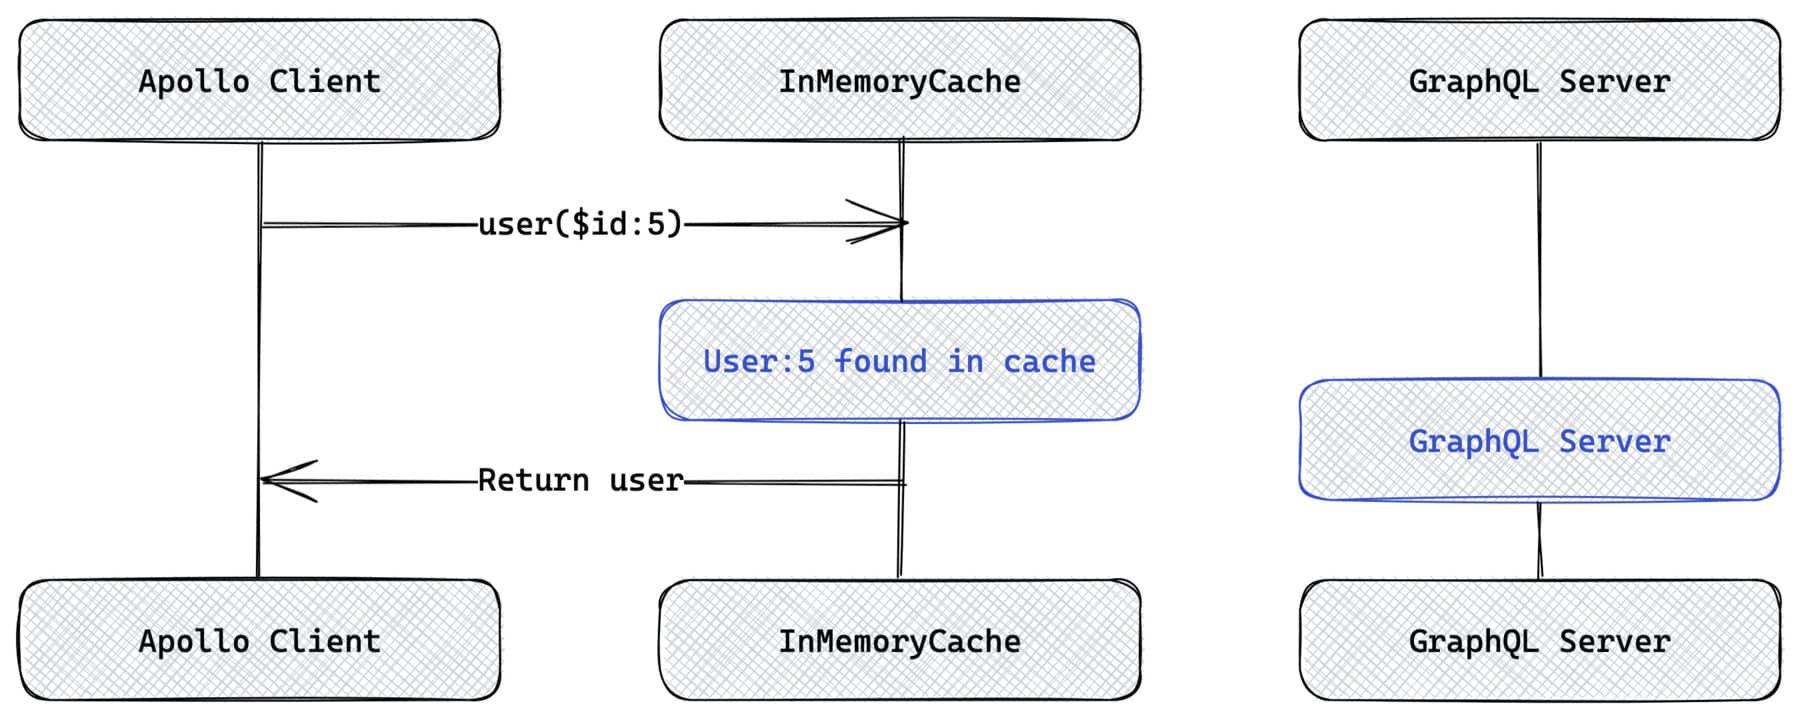
\includegraphics[width=0.7\linewidth]{images/background/graphql/apollo/apollo-client-basic-cache-warm.jpg}
  \caption{Execute the same query, which reduces the necessary steps. (Adapted from \cite{misc:-:background:graphql:apollo-client-cache-overview})}\label{fig:background:graphql:user-query-second-time}
\end{figure}
\fi

\subsubsection{Data normalization}\label{subsubsection:background:graphql:apollo-server-client:data-normalization}

Whenever the Apollo Client receives the response data of a query, it does the following. To correctly understand cache updates, it is essential to the structure of the cache before. The \texttt{InMemoryCache} is a simple normalized \ac{JS} object. The Apollo Client stores the data as a flat lookup table of objects referencing each other. An empty cache is just an empty object. These objects correspond to the objects that are returned by GraphQL queries. A single cache object might include fields fetched by multiple queries, allowing multiple queries to fetch different fields for the same object. \cite{misc:-:background:graphql:apollo-client-cache-overview} The following paragraphs describe the steps from a GraphQL query to the objects inside the cache.

\paragraph{1. Identify objects}\label{paragraph:background:graphql:apollo-server-client:data-normalization:identify-objects}

The cache identifies all distinct objects included in the query response. For example, take the query from Listing \ref{code:background:graphql:query-user-cache}, which returns the \texttt{id}, \texttt{username}, and \texttt{email} of every user.

\ifshowListings
\begin{listing}[H]
  \begin{minted}{typescript}
query {
  users {
    id
    username
    email
  }
}
  \end{minted}
  \caption{GraphQL query that fetches the id, username, and email of every user.}\label{code:background:graphql:query-user-cache}
\end{listing}
\fi

\noindent The server responds with the following response seen in Listing \ref{code:background:graphql:query-user-response-result}. The \texttt{\_\_typename} property is automatically appended to the query by the Apollo Client to identify the object.

\ifshowListings
\begin{listing}[H]
  \begin{minted}{typescript}
{
  users: [
    {
      __typename: 'User',
      id: '36bad921-8fcf-4f33-9f29-0d3cd70205c8',
      username: 'Florian',
      email: 'florian@test.io'
    },
    {
      __typename: 'User',
      id: 'a2096556-9a4e-4994-9de8-86c9e85ed6a1',
      username: 'Lisa',
      email: 'lisa@test.io'
    }
  ]
}
  \end{minted}
  \caption{The result of the GraphQL query from Listing \ref{code:background:graphql:query-user-cache}.}\label{code:background:graphql:query-user-response-result}
\end{listing}
\fi

The caching mechanism identifies the following objects to be cached.

\begin{itemize}
  \item A \texttt{User} with id \texttt{36bad921-8fcf-4f33-9f29-0d3cd70205c8}
  \item A \texttt{User} with id \texttt{a2096556-9a4e-4994-9de8-86c9e85ed6a1}
\end{itemize}

\paragraph{2. Generate cache IDs}\label{paragraph:background:graphql:apollo-server-client:data-normalization:generate-cache-ids}

After identifying all objects, the cache generates a cache ID for each object. A cache ID uniquely identifies a particular object while it is in the \texttt{InMemoryCache}.

\noindent So, the cache IDs for the objects from the previous section are:

\begin{itemize}
    \item \texttt{User:36bad921-8fcf-4f33-9f29-0d3cd70205c8}
    \item \texttt{User:a2096556-9a4e-4994-9de8-86c9e85ed6a1}
\end{itemize}

\noindent By default, an object's cache ID is concatenated with the object's \texttt{\_\_typename} and \texttt{id} (or \texttt{\_id}) fields. If the cache cannot generate a cache ID for a particular object, that object is directly stored inside its parent object and must be referenced via the parent. Therefore the cache is not always completely flat. This behavior is shown with the query in Listing \ref{code:background:graphql:no-id-query-user-cache}. 

\ifshowListings
\begin{listing}[H]
  \begin{minted}{typescript}
query {
  allUsers {
    id
    username
    Title {
      name
    }
  }
}
  \end{minted}
  \caption{Fetch the \texttt{id}, \texttt{username} and the \texttt{name} of the title of the user, without the \texttt{id} of the title.}\label{code:background:graphql:no-id-query-user-cache}
\end{listing}
\fi

\noindent The query from the listing misses the \texttt{id} field inside the Title field. Therefore the cache stores the Title object directly inside the user object. The result inside the cache is shown in the listing
\ref{code:background:graphql:no-id-query-user-cache-representation}. 

\ifshowListings
\begin{listing}[H]
  \begin{minted}{typescript}
{
  'User:36bad921-8fcf-4f33-9f29-0d3cd70205c8': {
    __typeName: 'User',
    id: '36bad921-8fcf-4f33-9f29-0d3cd70205c8',
    username: 'Florian',
    Title: { name: 'BSc.' }
  },
  'User:a2096556-9a4e-4994-9de8-86c9e85ed6a1': {
    __typeName: 'User',
    id: 'a2096556-9a4e-4994-9de8-86c9e85ed6a1',
    username: 'Lisa',
    Title: { name: 'BSc.' }
  }
}
  \end{minted}
  \caption{The content of the cache after fetching the query from Listing \ref{code:background:graphql:no-id-query-user-cache}.}\label{code:background:graphql:no-id-query-user-cache-representation}
\end{listing}
\fi

\noindent Omitting IDs from a query should be avoided. If data of an un-normalized object has to be updated, every occurrence of the item in the cache has to be updated manually. It should be avoided that the same thing is queried, sometimes with an id and sometimes without, because Apollo Client will throw an error when trying to update the cache after such a query.

\paragraph{3. Replace object fields with references}\label{paragraph:background:graphql:apollo-server-client:data-normalization:replace-object-fields-with-references}

Next, the cache takes each field that contains an object and replaces its value with a reference to the appropriate object. Listing \ref{code:background:graphql:nested-query-user-cache} shows a query that demonstrates how the objects from a query are transformed in the \texttt{InMemoryCache} representation.

\ifshowListings
\begin{listing}[H]
  \begin{minted}{typescript}
query {
  allUsers {
    id
    username
    Title {
      id
      name
    }
  }
}
  \end{minted}
  \caption{A GraphQL query to fetch all users.}\label{code:background:graphql:nested-query-user-cache}
\end{listing}
\fi

Listing \ref{code:background:graphql:nested-query-response-user-cache} shows a single result from the GraphQL server for the query from Listing \ref{code:background:graphql:nested-query-user-cache}.

\ifshowListings
\begin{listing}[H]
    \begin{minted}{typescript}
{
  __typename: 'User',
  id: '36bad921-8fcf-4f33-9f29-0d3cd70205c8',
  username: 'Florian',
  title: {
    __typename: 'Title',
    id: '2adb1120-d911-4196-ab1b-d5043cc7a00a',
    name: 'BSc.'
  }
}
    \end{minted}
    \caption{The result of the GraphQL query from Listing \ref{code:background:graphql:nested-query-user-cache}.} \label{code:background:graphql:nested-query-response-user-cache}
\end{listing}
\fi

\noindent And Listing \ref{code:background:graphql:nested-query-response-after-replacement} shows how the object is stored inside the \texttt{InMemoryCache}.

\ifshowListings
\begin{listing}[H]
  \begin{minted}{typescript}
{
  __typename: 'User',
  id: '36bad921-8fcf-4f33-9f29-0d3cd70205c8',
  username: 'Florian',
  title: { __ref: 'Title:36bad921-8fcf-4f33-9f29-0d3cd70205c8' }
}
  \end{minted}
  \caption{The structure of the cache after the user object is stored.}\label{code:background:graphql:nested-query-response-after-replacement}
\end{listing}
\fi

\noindent The \texttt{title} field now references the appropriate normalized \texttt{Title} object. If another \texttt{User} with the same \texttt{title} is stored inside the in-memory cache, that normalized \texttt{Title} object is reused. Normalization can drastically reduce data duplication inside the cache, and it also helps to make the data stay synchronous with the server.

\paragraph{4. Store normalized objects}\label{paragraph:background:graphql:apollo-server-client:data-normalization:store-normalized-objects}

The resulting objects are stored inside the cache's flat lookup table. Whenever an incoming object has the same cache ID as an existing cached object, the fields of those objects are merged. If the incoming and the existing object share existing fields, the incoming object overwrites the cached value for those fields. Fields that exist in only one object are preserved. This normalization constructs a partial copy of the graph on our client. \cite{misc:-:background:graphql:apollo-client-cache-overview}

\bigskip

\noindent Listing \ref{code:background:graphql:nested-query-user-cache-representation} shows how normalized objects are stored. Each user contains a reference to a title. Both users have the same title. Therefore the server returned duplicate data. However, the cache normalization causes the title to be only present once inside the cache. This behavior is constructive because when a cache item is updated, the entire cache object does not have to be traversed in search of the instance that has been changed. Only a single item has to be updated. The cache normalization works when the query contains either a \texttt{\_id} or \texttt{id} field.

\ifshowListings
\begin{listing}[H]
    \begin{minted}{typescript}
{
  'User:36bad921-8fcf-4f33-9f29-0d3cd70205c8': {
    __typeName: 'User',
    id: '36bad921-8fcf-4f33-9f29-0d3cd70205c8',
    username: 'Florian',
    Title: { __ref: 'Title:2adb1120-d911-4196-ab1b-d5043cc7a00a' },
  },
  'User:a2096556-9a4e-4994-9de8-86c9e85ed6a1': {
    __typeName: 'User',
    id: 'a2096556-9a4e-4994-9de8-86c9e85ed6a1',
    username: 'Lisa',
    Title: { __ref: 'Title:2adb1120-d911-4196-ab1b-d5043cc7a00a' },
  }
  'Title:2adb1120-d911-4196-ab1b-d5043cc7a00a': {
    __typeName: 'Title',
    id: '2adb1120-d911-4196-ab1b-d5043cc7a00a',
    name: 'BSc.',
  },
}
  \end{minted}
  \caption{The structure of the cache with the result from the query from Listing \ref{code:background:graphql:nested-query-user-cache}.}\label{code:background:graphql:nested-query-user-cache-representation}
\end{listing}
\fi

\subsubsection{Understanding the structure of the cache}\label{subsubsection:background:graphql:apollo-server-client:understanding-cache-structure}

Apollo Client offers development tools for the browser in the form of browser extensions. The Apollo Client Developer Tools\footnote{\url{https://chrome.google.com/webstore/detail/apollo-client-devtools/jdkknkkbebbapilgoeccciglkfbmbnfm}} can be installed for Chrome and Firefox. The extension can be found in the Chrome Web Store and the Firefox Add-ons Store. The browser extension adds a tab to the browser inspection tools. \cite{misc:-:background:graphql:apollo-developer-tools} The view of the cache contents from the Apollo Client Development Tools can be seen in Figure \ref{fig:background:graphql:apollo:apollo-dev-tools}.

\ifshowImages
  \begin{figure}[H]
    \centering
    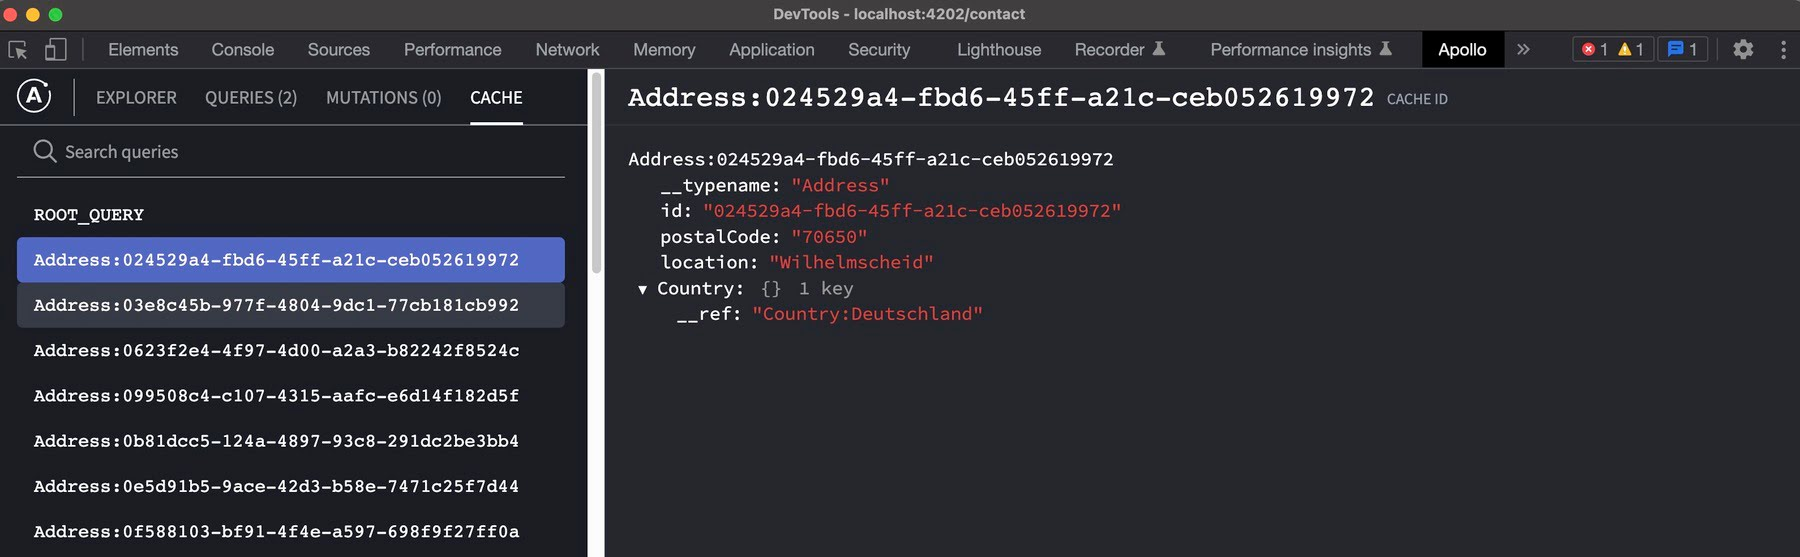
\includegraphics[width=1\linewidth]{images/background/graphql/apollo/apollo-dev-tools.jpg}
    \caption{The content of the cache inside the Apollo Client Developer Tools.}\label{fig:background:graphql:apollo:apollo-dev-tools}
  \end{figure}
\fi

\noindent The development tools offer the following four main features: \cite{misc:-:background:graphql:apollo-developer-tools}

\begin{itemize}
  \item \textbf{GraphiQL}: Send queries to the server through the web application's configured Apollo Client instance, or query the Apollo Client cache to see what data is loaded.
  \item \textbf{Watched query inspector}: View active queries, variables, cached results, and re-run individual queries.
  \item \textbf{Mutation inspector}: View active mutations and their variables, and re-run individual mutations.
  \item \textbf{Cache inspector}: Visualize the Apollo Client and search it by field name and/or value.
\end{itemize}

\noindent Another method to access the content of the cache is through the \texttt{window} object in \ac{JS}. The object can be accessed through \texttt{window.\_\_APOLLO\_CLIENT\_\_.cache.extract()} inside the browser's development tools. The result of this method invocation can be seen in Figure \ref{fig:background:graphql:apollo:apollo-cache-browser-window}.

\ifshowImages
  \begin{figure}[H]
    \centering
    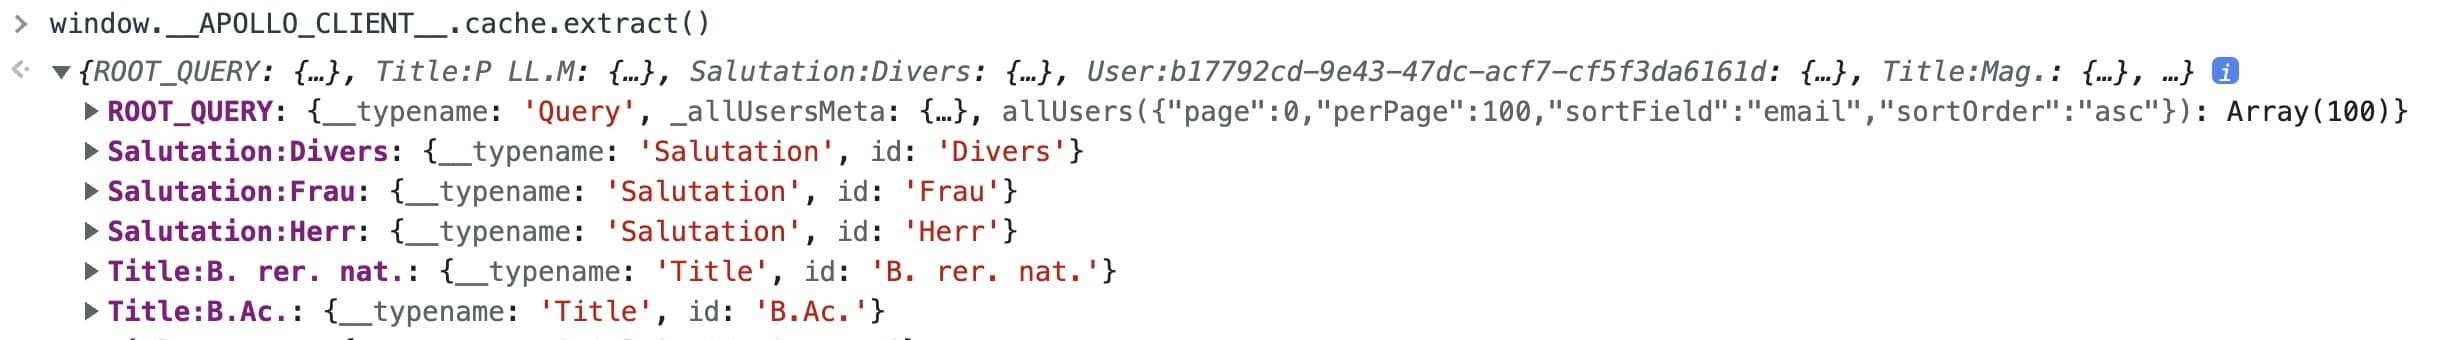
\includegraphics[width=1\linewidth]{images/background/graphql/apollo/apollo-cache-browser-window.jpg}
    \caption{View the content of the cache inside the development tools.}\label{fig:background:graphql:apollo:apollo-cache-browser-window}
  \end{figure}
\fi

\noindent With this approach, the content of the cache can be explored with the help of \ac{JS} methods inside the browser development tools.

\subsubsection{Type-Policies}\label{subsubsection:background:graphql:apollo-server-client:type-policies}

Type policies are a way to define how the client stores and manages data in the cache. The constructor of the \texttt{InMemoryCache} accepts type policies as an object. The \texttt{typePolicies} object the behavior of the cache can be customized on a type-by-type basis. Type policies are fine-grained; they allow to customize how a specific field inside the cache is read and written. A type policy contains multiple field policies that customize the behavior of the fields for that type. \cite{misc:-:background:graphql:apollo-client-cache-reading-writing}

\bigskip

\noindent A field policy for a field consists of: \cite{misc:-:background:graphql:apollo-client-cache-reading-writing}

\begin{itemize}
  \item A \texttt{read} function which is called when the field is read from the cache.
  \item A \texttt{merge} function which is called when the field is written to the cache.
  \item An array of fields, which are the key arguments that identify an object. This so-called \texttt{keyArgs} avoids storing duplicate data in the cache.
\end{itemize}

\paragraph{Read function}

Listing \ref{code:background:graphql:read-type-policy} shows the definition of a \texttt{read} function. The cache calls that function when the client queries for a user's first name. The \texttt{InMemoryCache} then returns the function's response instead of the cached value. The first parameter of the function is the current value of the field. The second parameter is an object that contains the arguments of the field and several helper functions and properties. \cite{misc:-:background:graphql:apollo-client-cache-reading-writing} The \texttt{read} function of Listing \ref{code:background:graphql:read-type-policy} returns a default value for the \texttt{firstName} of the \texttt{User} type when a value is unavailable in the cache. If a value exists in the cache, the value is returned unmodified.

\ifshowListings
\begin{listing}[H]
    \begin{minted}{typescript}
new InMemoryCache({
  typePolicies: { User: { fields: {
    firstName: {
      read(value, options) {
        return value ?? 'Unknown';
      }
    }
  }}}
});
    \end{minted}
    \caption{Provide a default value for the  \texttt{firstName} field.}\label{code:background:graphql:read-type-policy}
\end{listing}
\fi

\paragraph{Merge function}

The \texttt{merge} function for a field is called whenever the field is about to be written with an incoming value. The field's new value is set to the \texttt{merge} function's return value instead of the original value.  An everyday use case for the \texttt{merge} function is to define a field policy for a field that holds an array. By default, the existing collection is completely replaced by the incoming array. However, sometimes, both arrays should be concatenated. This pattern is used with paginated lists, where the incoming page should be merged with the existing pages. The parameters are the current value, the incoming value, and the options, just like in the \texttt{read} function. \cite{misc:-:background:graphql:apollo-client-cache-reading-writing}

\bigskip

\noindent Listing \ref{code:background:graphql:write-type-policy} shows the definition of a \texttt{merge} function. Whenever a new transaction for the bank account is fetched, the existing and the incoming transactions are merged. Initially, \texttt{existing} is undefined; therefore, \texttt{existing} is assigned a default parameter.

\ifshowListings
\begin{listing}[H]
    \begin{minted}{typescript}
new InMemoryCache({
  typePolicies: { BankAccount: { fields: {
    transaction: {
      merge(existing = [], incoming: unknown[], options) {
        return [...existing, ...incoming];
      },
    },
  }}},
});
    \end{minted}
    \caption{Merge the existing and incoming transactions in a \texttt{merge} function.}\label{code:background:graphql:write-type-policy}
\end{listing}
\fi

\subsection{Query Reduction}

This section describes the theory behind reducing queries with already existing data inside the cache. Apollo Client does not offer this behavior by default. The Github repository features a lot of feature requests that want such a feature implemented for queries. Unfortunately this did not happen. The next section describes how the theory behind reduction works.

\subsubsection{Theoretical Concept}

In large applications, it is likely that the same query is executed with different selection sets over and over again. Unless the selection set of the query is perfectly identical, Apollo Client will fetch the query from the server. Ignoring the fact that many of the queries fields are already inside the cache. An example query is shown in listing \ref{code:background:graphql:query-reduction:example-query-simple}

\ifshowListings
\begin{listing}[H]
\begin{minted}{typescript}
query {
  allUsers {
    id
    username
    Title {
      id
      name
    }
  }
  allTitles {
    id
    name
  }
}
\end{minted}
\caption{An exemplary GraphQL query that fetches all users}\label{code:background:graphql:query-reduction:example-query-simple}
\end{listing}
\fi

The first time this query is executed, a request is sent to the server. Each subsequent execution of the query with the same selection set is served from the cache and a round trip to the server is saved. Afterwards the same query is executed with a different selection set. The query is sent to the server again, even though the selection set is only slightly different. The selection set of the query is extended by the email field and is shown in listing \ref{code:background:graphql:query-reduction:example-query-extended}

\ifshowListings
\begin{listing}[H]
\begin{minted}{typescript}
query {
  allUsers {
    id
    username
    email // Additional field
    Title {
      id
      name
    }
  }
  allTitles {
    id
    name
  }
}
\end{minted}
\caption{An exemplary GraphQL query that fetches all users with an additional field}\label{code:background:graphql:query-reduction:example-query-extended}
\end{listing}
\fi

The queries are almost identical, but there is an additional field, this will result in a cache miss. The entire query will be requested from the server. This is quite unnecessary because the most part of the data is already in the cache. A better approach would be to fetch only the field which is missing inside the cache like shown in \ref{code:background:graphql:query-reduction:example-query-reduced}.

\ifshowListings
\begin{listing}[H]
\begin{minted}{typescript}
query {
  allUsers {
    id
    email
  }
}
\end{minted}
\caption{The part of the exemplary query that is necessary}\label{code:background:graphql:query-reduction:example-query-reduced}
\end{listing}
\fi

The id can't be removed from the query as it needed to merge the existing and incoming data together afterwards. Depending how many shared selections exist inside the application's queries, a lot of server resources can be saved by reducing the queries. 



